\section{Uso de Seções}

A apresentação deve ser dividida em seções. As seções são apresentadas na agenda, e, de preferência, devem variar entre 5 e 7, não sendo menos que 3 e não ultrapassando 9.

Na maioria das apresentações, duas seções são essenciais: introdução e conclusão. Algumas coisas também não precisam ter seções indicadas, como a Bibliografia e, quando existir, a apresentação do autor, autores ou grupo de pesquisa.

Cada seção deve possuir uma capa, na forma de título ou de uma versão da agenda. A Figura \ref{fig:meio} mostra um slide com uma versão da agenda levemente modificada por meio do uso de sombra nos itens já tratados, que é criada automaticamente no \texttt{beamer} com os comandos que aparecem na Listagem \ref{fig:autosec}.

\begin{figure}[hb]
    \centering
    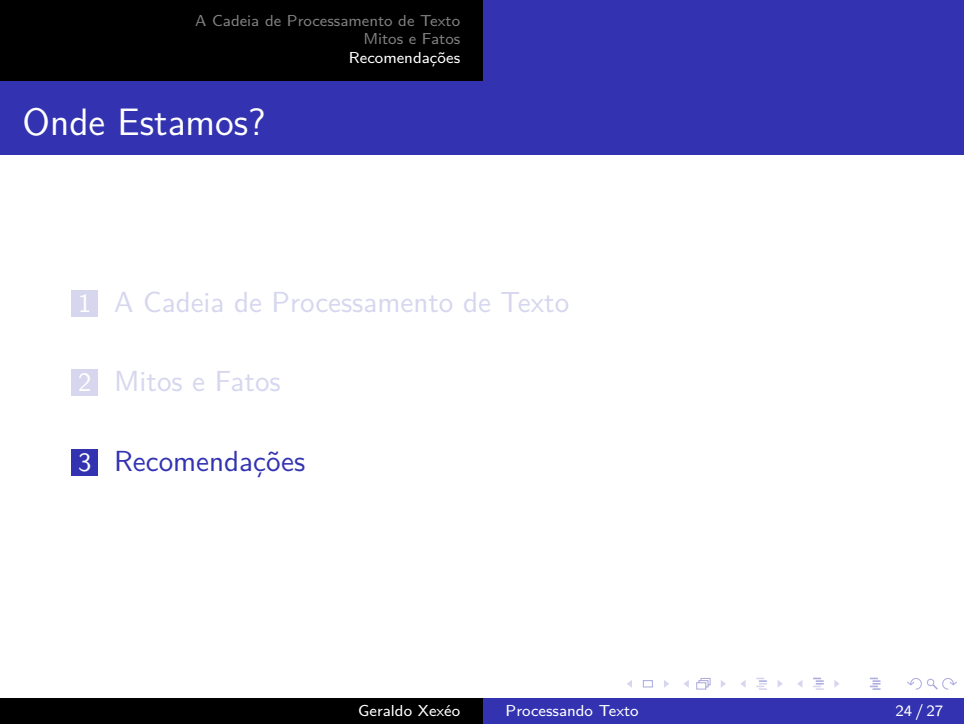
\includegraphics[width=\tam\linewidth,frame]{imagens/agendadomeio.png}
    \caption{Um slide mostrando a parte que será falada da agenda, com as outras partes acinzentadas. Criada usando o \LaTeX\  e o \texttt{beamer}.}
    \label{fig:meio}
\end{figure}

\begin{lstlisting}[language=TeX,caption={Comando para títulos de seção automáticos no \texttt{beamer} com o tema Luebeck.},label={lst:autosec}]
\AtBeginSection[]
{\begin{frame}
   \frametitle{Onde Estamos?}
     \tableofcontents[currentsection,hideallsubsections ]
 \end{frame}}
\end{lstlisting}

Um título de seção pode ter vários formatos, a Figura \ref{fig:sectitles} mostra um simples e três variações que experimentei em aulas diferentes.

\begin{figure}
    \centering
        \subfloat{
        
\includegraphics[width=0.4\linewidth,frame]{imagens/sec1}
    }
    \subfloat{
    
\includegraphics[width=0.4\linewidth,frame]{imagens/valor}
}\\
    \subfloat{
        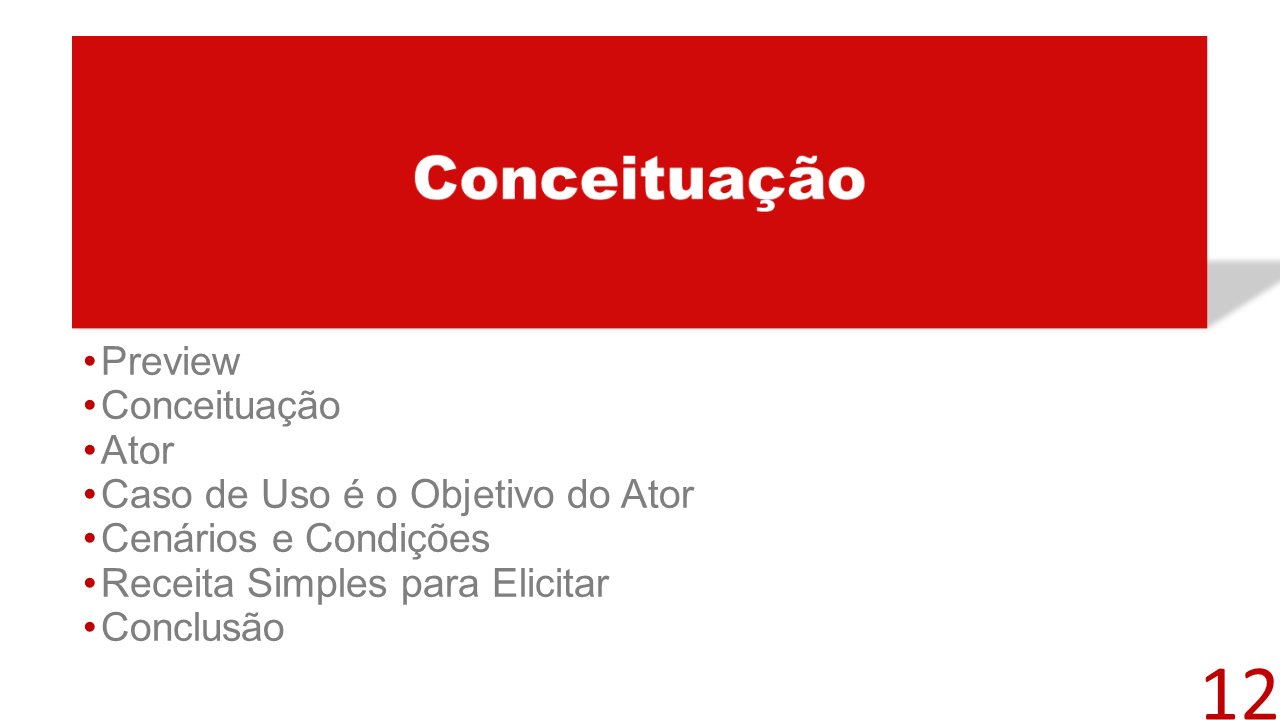
\includegraphics[width=0.4\linewidth,frame]{imagens/casosdeuso}
    }
    \subfloat{
    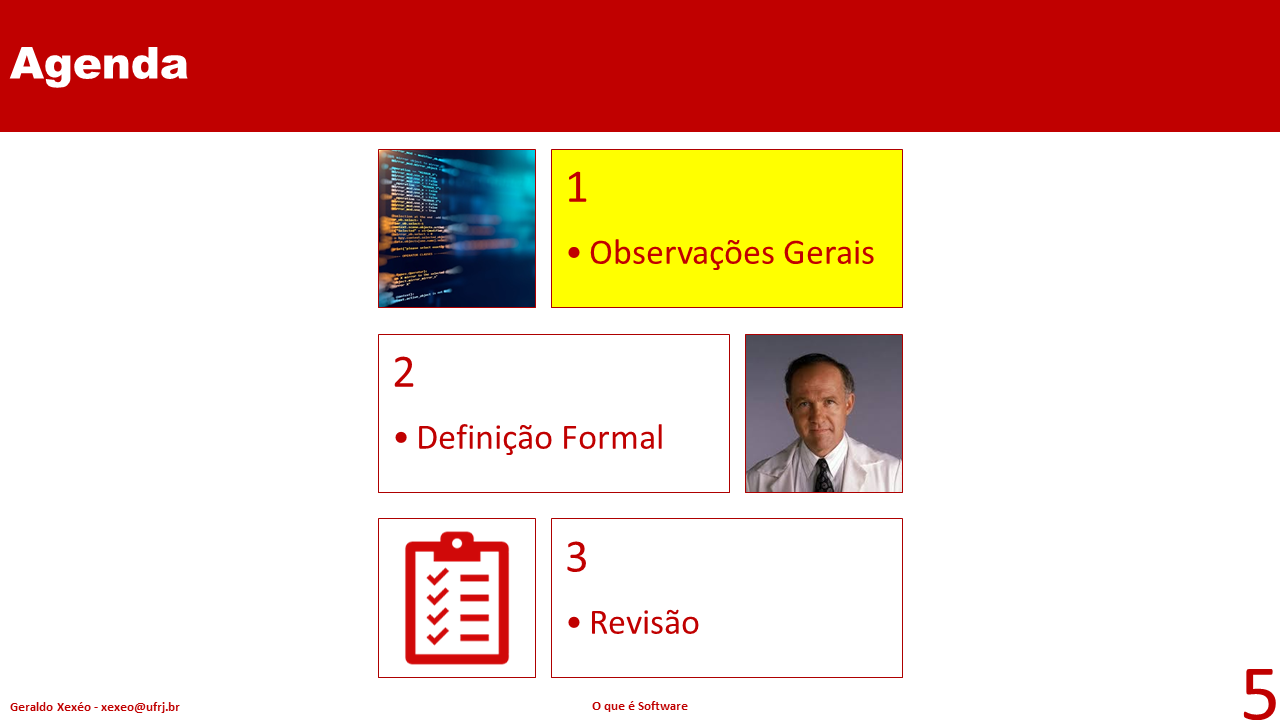
\includegraphics[width=0.4\linewidth,frame]{imagens/sec2}
}
\caption{Várias formas de fazer um título de seção}.
\label{fig:sectitles}
\end{figure}


